\chapter{Ответы}
\label{ch:answers}

\openepigraph{%
Ставлю три звездочки. 
Я видал в детских книжках: 
когда человек делает прыжок к новой мысли, он ставит три звездочки\ldots
}{Саша Чёрный, {Дневник Фокса Микки}%
}

\newthought{Задачи рассеяны} по всей книге, а ответы на них собраны в этом разделе.

\begin{task}
    \label{answer:instance-in-OOP-vs-Wikidata}
    \newthought{Экземпляр объекта}\footnote[][0cm]{См. статью 
        \href{https://en.wikipedia.org/wiki/Instance\_(computer\_science)}{Instance (computer science)} в Английской Википедии.
                                                  }%
    в Викиданных 
    и в объектно-ориентированном программировании (ООП) сходны в сути, а именно:
    есть модель базового объекта $D$, создаётся новая единица $I$, обладающая 
    свойствами той же модели $D$. 
    В программировании о создании $I$ говорят, 
    что класс $D$ проинициализирован 
    и получен объект $I$\footnote[][0cm]{%
        $I$~является экземпляром $D$ или 
        \mbox{$I$~is instance of $D$} по-английски.}. 
%        $I$~is instance of $D$ по-английски, 
%        $I$~является экземпляром $D$ \mbox{по-русски}}.

    В чём разница? 
    В ООП в исходном коде программы мы видим как во времени последовательно 
    (в разных строках программы) происходит 
    объявление переменной, инициализация класса, 
    присвоение значений экземплярам класса.
    В Викиданных в тот момент, когда выполняется скрипт и происходит обращение 
    к данным, объекты, являющиеся экземплярами других объектов, 
    уже представлены и обычно не происходит их изменение, 
    связанное с работой SPARQL-скриптов.

    \small{Вопрос на с.~\pageref{question:instance-in-OOP-vs-Wikidata}.}
\end{task}


\begin{task}
    \label{answer:guess_numbers_task}
    \newthought{В алгоритме угадывания чисел} число $ a $ может быть натуральным, целым, вещественным и рациональным числом, то есть $ a \in \mathbb{N},\mathbb{Z}, \mathbb{Q}, \mathbb{R} $, но кроме иррациональных чисел из-за конечности разрядной сетки компьютера. 
    \small{Вопрос на с.~\pageref{question:text}}
\end{task}

\begin{task}
    \label{answer:global-vars-pros-cons}
    \newthought{Ответ такой} ... todo. 

    \small{Вопрос на с.~\pageref{fig:block:proc:swap:colors}.}
\end{task}

%%%%%%%%%%%%%% City chapter %%%%%%%%%%%%%%
\begin{task}
    \label{answer:cities_geographic_objects}
    \newthought{В честь географических объектов} были названы Тула (\href{https://w.wiki/oLJ}{река Тулица}), Курильск (\href{https://w.wiki/oLH}{Курильские острова}) и Вологда (\href{https://w.wiki/oLG}{река Вологда}). Ответ на вопрос также можно получить, выполнив следующий SPARQL-запрос (листинг \ref{lst:cities_geographic_objects}). Значение свойства \href{https://www.wikidata.org/wiki/Property:P138}{named after (P138)} показывает, в честь какого объекта Викиданных был назван город.
    
    \marginnote[-1.0cm]{
    Поясним вторую строчку скрипта в листинге \ref{lst:cities_geographic_objects}, то есть конструкцию wdt:P31/wdt:P279*, за которой следует объект Викиданных, объединяющий \wdqName{city}{515} и \wdqName{town}{3957}, и называющийся \wdqName{city/town}{7930989}.
    Если не имеет значения к какому конкретно типу городов относится объект Викиданных, то можно использовать конструкцию с подклассами, указав при этом единственный класс, относительно которого будет выполняться поиск. Более подробно данная конструкция рассматривается в разделе <<Полнота и недостатки Викиданных>>, в тексте, предшествующем листингу \ref{lst:example_subclasses_city} на с. \pageref{lst:example_subclasses_city}.
    }
    
    \index{SPARQL!FILTER!Города, названные в честь географических объектов}
    \begin{lstlisting}[ language=SPARQL, 
                    caption={\href{https://w.wiki/otj}{Города, названные в честь географических объектов}\protect\footnotemark},
                    label=lst:cities_geographic_objects
                    ]
SELECT ?city ?cityLabel ?namedAfterLabel ?whatIsItLabel WHERE {
	?city wdt:P31/wdt:P279* wd:Q7930989. # "city/town" subclasses
	?city wdt:P138 ?namedAfter. # with filled property "named after"
	?namedAfter wdt:P31 ?whatIsIt. # which is instance of
	FILTER(?city = wd:Q1341 || ?city = wd:Q2770 || ?city = wd:Q5655 ||
		?city = wd:Q156046 || ?city = wd:Q1957 || ?city = wd:Q175651)
	SERVICE wikibase:label { bd:serviceParam wikibase:language "ru" }
}
    \end{lstlisting}
    \footnotetext{Ссылка на SPARQL-запрос: \href{https://w.wiki/otj}{https://w.wiki/otj}}  
    \small{Вопрос на с.~\pageref{lst:population_town}.}
\end{task}

\begin{task}
    \label{answer:cities_over_400_age}
    \newthought{Более 400 лет назад} были основаны Казань (1005 год), Москва (1147), Астрахань (1558), Воронеж (1586) и Самара (1586). Самым молодым городом оказался Саров, основанный в 1691 году. Ответ на вопрос также можно получить, выполнив следующий SPARQL-запрос (листинг \ref{lst:cities_over_400_age}). Значение свойства \href{https://www.wikidata.org/wiki/Property:P571}{inception (P571)} содержит дату основания города.

\marginnote{
Какие строчки в листинге \ref{lst:cities_over_400_age} нужно закомментировать, чтобы:
\begin{itemize}
	\item[а)] получить список всех отечественных городов, основанных более 400 лет назад?
	\item[б)] получить список всех городов мира, основанных в те же годы?
\end{itemize}
}

\marginnote[0.5cm]{
Может ли в листинге \ref{lst:cities_over_400_age} переменная ?year принимать отрицательные значения? Почему?
}
    
    \index{SPARQL!FILTER!Города, основанные более 400 лет назад}
    \index{SPARQL!YEAR!Города, основанные более 400 лет назад}
    \begin{lstlisting}[ language=SPARQL, 
                    caption={\href{https://w.wiki/t5u}{Города, основанные более 400 лет назад}\protect\footnotemark},
                    label=lst:cities_over_400_age
                    ]
SELECT ?city ?cityLabel (YEAR(?inceptionDate) AS ?year) WHERE {
	?city wdt:P31/wdt:P279* wd:Q7930989. # "city/town" subclasses
	?city wdt:P17 wd:Q159. # belonging to Russia
	?city wdt:P571 ?inceptionDate. # with filled property "inception"  
	FILTER (YEAR(?inceptionDate) < 1620). # 2020 - 400 years
	FILTER(?city = wd:Q649 || ?city = wd:Q193522 || ?city = wd:Q900 ||
		?city = wd:Q3927 || ?city = wd:Q894 || ?city = wd:Q3426)
	SERVICE wikibase:label { bd:serviceParam wikibase:language "ru" }
}
GROUP BY ?city ?cityLabel ?inceptionDate
ORDER BY ASC(?year)
\end{lstlisting}
\footnotetext{Ссылка на SPARQL-запрос: \href{https://w.wiki/t5u}{https://w.wiki/t5u}} 

У объекта Викиданных \wdqName{Москва}{649} свойство \href{https://www.wikidata.org/wiki/Property:P571}{inception} принимает значение <<unknown value>> (неизвестное значение) с квалификатором <<самое позднее упоминание>> (\href{https://www.wikidata.org/wiki/Property:P1326}{latest date}) = 4 апреля 1147 года. Вероятно, по этой причине в листинге \ref{lst:cities_over_400_age} переменная ?year принимает для Москвы пустое значение, и Москва ошибочно не попадает в список правильных ответов. Таким образом, чтобы извлечь 1147 год, необходимо доработать имеющийся скрипт, что мы оставим читателю. 

\marginnote[-1.0cm]{
О типах данных и наборах свойств, связанных с датой и временем, см. \href{https://w.wiki/NdT}{Help:Dates}.
}


    \small{Вопрос на с.~\pageref{fig:city_relation_Russia_S_N}.}
\end{task}

\begin{task}
    \label{answer:cities_flags}
    \newthought{Флаг, изображенный на рис. \ref{fig:flag_question_city}} принадлежит городу \href{https://w.wiki/oLF}{Карабулак}. Ответ на вопрос также можно получить, выполнив следующий SPARQL-запрос (листинг \ref{lst:cities_flags}). Значение свойства \href{https://www.wikidata.org/wiki/Property:P41}{flag image (P41)} содержит изображение флага города.
    
    \index{SPARQL!FILTER!Флаги городов}
    \begin{lstlisting}[ language=SPARQL, 
                    caption={\href{https://w.wiki/t5q}{Флаги городов}\protect\footnotemark},
                    label=lst:cities_flags
                    ]
#defaultView:ImageGrid
SELECT ?city ?cityLabel ?flag ?countryLabel WHERE {
	?city wdt:P31/wdt:P279* wd:Q7930989. # "city/town" subclasses
	?city wdt:P17 wd:Q159. # belonging to Russia	
	?city wdt:P41 ?flag. # with filled property "flag"
	SERVICE wikibase:label { bd:serviceParam wikibase:language "ru" }
}
\end{lstlisting}
\footnotetext{Ссылка на SPARQL-запрос: \href{https://w.wiki/t5q}{https://w.wiki/t5q}}  
    
    \small{Вопрос на с.~\pageref{lst:countries_sister_cities_with_Russia}.}
\end{task}

%%%%%%%%%%%%%% Country chapter %%%%%%%%%%%%%%

\begin{task}
	\label{answer:administrative_territorial}
	\newthought{ 
		Речь идет о количестве административно-территориальных единиц в каждой из стран. 
		%Количество административно-территориальных единиц у \href{https://w.wiki/mzN}{Латвии}  119, у \href{https://w.wiki/mzP}{Таиланда} 77, у \href{https://w.wiki/mzR}{Дании} 5, а у \href{https://w.wiki/myt}{России} 81. 
		Ответ на вопрос можно проверить, выполнив следующий SPARQL-запрос (листинг \ref{lst:administrative_territorial_entity}).}
	
	\begin{lstlisting}[ language=SPARQL, 
	caption={\href{https://w.wiki/tiN}{
	Список стран, упорядоченных по количеству административно-территориальных единиц}\protect\footnotemark},
	label=lst:administrative_territorial_entity	]
# Countries sorted by number of administrative territories
SELECT ?country ?countryLabel  (count(*) as ?count)
WHERE
{
	?country p:P31 [ps:P31 wd:Q6256].# is a country
	?country wdt:P150 []. # has some administrative territory
	SERVICE wikibase:label { bd:serviceParam wikibase:language "ru" }
}
GROUP BY ?country ?countryLabel
ORDER BY DESC(?count)
	\end{lstlisting}
	\footnotetext{Получено 199 стран на 2021 год. Ссылка на SPARQL-запрос: \href{https://w.wiki/tiN}{https://w.wiki/tiN}}  
	
	\small{Вопрос на с.~\pageref{lst:age_of_country}.}
\end{task}

\begin{task}
	\label{answer:old_countries}
	\newthought{ 
		Результатом работы скрипта (листинг \ref{lst:old_countries}) будет список империй и небольших стран, исчезнувших с лица земли. Две с половиной тысячи лет и больше просуществовали только семь государств: \href{https://w.wiki/vAT}{Угарит} (4810 лет), \href{https://w.wiki/vAU}{Тамла} (3740 лет), \href{https://w.wiki/vAX}{Древний Египет} (3544 лет), \href{https://w.wiki/vAY}{Майя} (3521 год), \href{https://w.wiki/vAZ}{Идалион} (2550 год), \href{https://w.wiki/vAb}{Мероитское царство} (2529 год) и город-государство \href{https://w.wiki/vAf}{Дильмун} (2500 лет).
	}
\index{SPARQL!FILTER EXISTS!Страны, отсортированных по дате основания}
	\begin{lstlisting}[ language=SPARQL, 
	caption={\href{https://w.wiki/tYc}{
	Список исторических стран, отсортированных по дате основания}\protect\footnotemark},
	label=lst:old_countries	]
	# List of historical countries sorted by inception date
	SELECT ?country ?countryLabel 
	(MIN(?start) AS ?min_year)
	(MAX(?end)   AS ?max_year) 
	(?max_year - ?min_year as ?age)
	WHERE
	{
	?country p:P31 [ps:P31 wd:Q3024240]. # instance of a historical country
	
	FILTER EXISTS {?country wdt:P571 []}.# skip countries without inception date
	FILTER EXISTS {?country wdt:P576 []}.# skip countries without dissolution date
	
	OPTIONAL {?country p:P571 [ps:P571 ?inception].}# any inception date
	OPTIONAL {?country p:P576 [ps:P576 ?dissolution].}# any dissolution date
	
	BIND(YEAR(?inception) AS ?start)
	BIND(YEAR(?dissolution) AS ?end)  
	SERVICE wikibase:label { bd:serviceParam wikibase:language "ru,[AUTO_LANGUAGE],en" }
	}
	GROUP BY ?country ?countryLabel ?min_year ?max_year ?age
	ORDER BY DESC(?age)
	\end{lstlisting}
	\footnotetext{Ссылка на SPARQL-запрос: \href{https://w.wiki/tYc}{https://w.wiki/tYc}}  
	
	\small{Вопрос на с.~\pageref{lst:List_of_historical_countries}.}
\end{task}

\begin{task}
	\label{answer:population_density}
	\newthought{ Площадь Израиля составляет \num{20770} км\begin{math}^2\end{math}, население  \num{9.09} млн человек, площадь Монголии составляет  \num{1566000} км\begin{math}^2\end{math}, население  \num{3.08} млн человек, площадь Республики Кореи составляет \num{100295} км\begin{math}^2\end{math}, население  \num{51.47} млн человек, а площадь Сингапура~--- \num{719.1} км\begin{math}^2\end{math}, население  \num{5.89} млн человек. Таким образом, по возрастанию плотности населения страны будут упорядочены так:
		\begin{enumerate}
			\item Монголия (\num{1.96} человек на км\begin{math}^2\end{math}), (рис.~\ref{fig:flag_mongolia});
			\item Израиль (\num{437.79} человек на км\begin{math}^2\end{math}), (рис.~\ref{fig:flag_israel});
			\item Корея (\num{513.15} человек на км\begin{math}^2\end{math}), (рис.~\ref{fig:flag_kor});
			\item Сингапур (\num{8189.30} человек на км\begin{math}^2\end{math}), (рис.~\ref{fig:flag_singapore}).
		\end{enumerate}	
	}
	
	
	\newthought{  Ответ на вопрос можно проверить, выполнив следующий SPARQL-запрос (листинг \ref{lst:population_density}).}
	
	\begin{marginfigure}[0.0cm]
		{
			\setlength{\fboxsep}{0pt}%
			\setlength{\fboxrule}{1pt}%
			\fcolorbox{gray}{gray}{
\includegraphics[width=\linewidth]{./chapter/country/256px-Flag_of_Mongolia.png}}%
		}
		\caption{Флаг \href{https://w.wiki/mze}{Монголии}.}%
		\label{fig:flag_mongolia}%
	\end{marginfigure}
	\begin{marginfigure}[0.0cm]
		{
			\setlength{\fboxsep}{0pt}%
			\setlength{\fboxrule}{1pt}%
			\fcolorbox{gray}{gray}{
\includegraphics[width=\linewidth]{./chapter/country/256px-Flag_of_Israel.png}}%
		}
		\caption{Флаг \href{https://w.wiki/mzh}{Израиля}.}%
		\label{fig:flag_israel}%
	\end{marginfigure}
	\begin{marginfigure}[0.0cm]
		{
			\setlength{\fboxsep}{0pt}%
			\setlength{\fboxrule}{1pt}%
			\fcolorbox{gray}{gray}{
\includegraphics[width=\linewidth]{./chapter/country/256px-Flag_of_South_Korea.png}}%
		}
		\caption{Флаг \href{https://w.wiki/mzc}{Республики Кореи}.}%
		\label{fig:flag_kor}%
	\end{marginfigure}
	\begin{marginfigure}[0.0cm]
		{
			\setlength{\fboxsep}{0pt}%
			\setlength{\fboxrule}{1pt}%
			\fcolorbox{gray}{gray}{
\includegraphics[width=\linewidth]{./chapter/country/256px-Flag_of_Singapore.png}}%
		}
		\caption{Флаг \href{https://w.wiki/mzd}{Cингапура}.}%
		\label{fig:flag_singapore}%
	\end{marginfigure}
	
	\begin{lstlisting}[ language=SPARQL, 
	caption={\href{https://w.wiki/tkD}{
	Плотность населения в странах Азии}\protect\footnotemark},
	label=lst:population_density
	]
# Population density in Asian countries
SELECT ?country ?countryLabel ?flag ?area ?population 
(?population / ?area as ?populationDensity)
{
	?country p:P31 [ps:P31 wd:Q6256].# this is a country
	?country wdt:P30 wd:Q48 .   # on the Asian continent 
	?country wdt:P41 ?flag .    # has flag
	?country wdt:P2046 ?area .  # has area
	?country wdt:P1082 ?population. # has population  
	SERVICE wikibase:label {bd:serviceParam wikibase:language "ru"}
}
ORDER BY DESC(?populationDensity)
	\end{lstlisting}
	\footnotetext{Получено 53 страны в 2020 году. Ссылка на SPARQL-запрос: \href{https://w.wiki/tkD}{https://w.wiki/tkD}}  
	
	
		\newthought{Результаты работы вы можете увидеть в виде <<плиточки>> из флагов. Для этого на странице \emph{Wikidata Query Service} под кнопкой запуска скрипта в выпадающем списке выберите \index{Wikidata Query Service!Image grid} \emph{Image grid}.}
	
	\small{Вопрос на с.~\pageref{lst:without_inception}.}
\end{task}

\begin{task}
	\label{answer:official_language}
	\newthought{Официальными языками \href{https://w.wiki/myt}{России} являются \href{https://w.wiki/myv}{абазинский}, \href{https://w.wiki/myx}{мокшанский} и \href{https://w.wiki/myy}{эрзянский} языки.  Ответ на вопрос можно проверить, выполнив следующий SPARQL-запрос (листинг \ref{lst:official_languages}).}
	
	\index{SPARQL!FILTER!Официальные языки в России}
	\begin{lstlisting}[ language=SPARQL, 
	caption={\href{https://w.wiki/tky}{Официальные языки в России}\protect\footnotemark},
	label=lst:official_languages
	]
# Official languages in Russia
SELECT ?lanquage ?lanquageLabel
WHERE
{ # Russia has the official language
	wd:Q159 p:P37 [ps:P37 ?lanquage].
	SERVICE wikibase:label {bd:serviceParam wikibase:language "ru"}
} ORDER BY ?lanquageLabel
	\end{lstlisting}
	\footnotetext{Получено 37 языков в 2020 году. Ссылка на SPARQL-запрос: \href{https://w.wiki/tky}{https://w.wiki/tky}}  
	
	\small{Вопрос на с.~\pageref{lst:List_of_historical_countries}.}
\end{task}

%%%%%%%%%%%%%% oblast_of_Russia %%%%%%%%%%%%%%

\begin{task}
	\label{answer:subjects_of_Russia_3}
	\newthought{Приведённому описанию соответствует флаг Московской области. Ответ на вопрос можно проверить, выполнив следующий SPARQL-запрос (листинг \ref{lst:subjects_of_Russia_3_q})}
	
	\begin{lstlisting}[ language=SPARQL, numbers=none,
	caption={\href{https://w.wiki/4cPg}{Флаги субъектов России.}\protect\footnotemark},
	label=lst:subjects_of_Russia_3_q
	]
# List of flags of the subjects of Russia
#defaultView:ImageGrid
SELECT ?subject ?subjectLabel ?flag
WHERE
{
  { ?subject wdt:P31 wd:Q835714 } UNION  # Oblast of Russia
  { ?subject wdt:P31 wd:Q41162 } UNION  # Republic of Russia
  { ?subject wdt:P31 wd:Q183342 } UNION  # Federal city of Russia
  { ?subject wdt:P31 wd:Q831740 } UNION  # Krai of Russia
  { ?subject wdt:P31 wd:Q309166 } UNION # Autonomus oblast of Russia
  { ?subject wdt:P31 wd:Q184122 } # Autonomus okrug of Russia
  
  SERVICE wikibase:label { bd:serviceParam wikibase:language "ru" }
   
  ?subject wdt:P41 ?flag
}
\end{lstlisting}
\footnotetext{Получено 86 записей в 2021 году. Ссылка на SPARQL-запрос: \href{https://w.wiki/4cPg}{https://w.wiki/4cPg}}  
	
\small{Вопрос на с.~\pageref{lst:oblast-of-Russia}.}
\end{task}

\begin{task}
	\label{answer:subjects_of_Russia_1}
	\newthought{Такой регионом является Карелия. Она расположена на северо-западе России, возникла в \num{1920} году. Она граничит с Ленинградской, Вологодской, Архангельской и Мурманской областью. Также граничит с Финляндией на западе.  Ответ на вопрос можно проверить, выполнив следующий SPARQL-запрос (листинг \ref{lst:sharesBorderWith}).}
	
	\begin{marginfigure}[0.0cm]
{
	\setlength{\fboxsep}{0pt}%
	\setlength{\fboxrule}{1pt}%
	
\includegraphics[width=0.8\linewidth]{"chapter/oblast_of_Russia/Flag_of_Karelia.png"}
}
\caption [Флаг Карелии, Россия.]{Флаг Карелии.}%
\label{fig:Flag_of_Karelia}%
\end{marginfigure}
	
	\begin{lstlisting}[ language=SPARQL, numbers=none,
	caption={\href{https://w.wiki/4cPh}{Границы и дата возникновения субъектов РФ}\protect\footnotemark},
	label=lst:sharesBorderWith
	]
# Borders and date of origin of the subjects of the Russian Federation
SELECT  ?subject ?subjectLabel 
        ?sharesBorderWith 
        ?sharesBorderWithLabel ?year
WHERE
{
  { ?subject wdt:P31 wd:Q835714 } UNION  # Oblast of Russia
  { ?subject wdt:P31 wd:Q41162 } UNION  # Republic of Russia
  { ?subject wdt:P31 wd:Q183342 } UNION  # Federal city of Russia
  { ?subject wdt:P31 wd:Q831740 } UNION  # Krai of Russia
  { ?subject wdt:P31 wd:Q309166 } UNION # Autonomus oblast of Russia
  { ?subject wdt:P31 wd:Q184122 } # Autonomus okrug of Russia
  
  SERVICE wikibase:label { bd:serviceParam wikibase:language "ru" }
  
  ?subject wdt:P47 ?sharesBorderWith. 
  ?subject wdt:P571 ?year
}
\end{lstlisting}
\footnotetext{Получено 485 записей в 2021 году. Ссылка на SPARQL-запрос: \href{https://w.wiki/4cPh}{https://w.wiki/4cPh}}  
	
\small{Вопрос на с.~\pageref{lst:sharesBorderWith-oblast-of-Russia}.}
\end{task}

\begin{task}
	\label{answer:subjects_of_Russia_2}
	\newthought{Сейчас в состав Российской Федерации входят: Республика Адыгея, Камчатский край, Чукотский автономный округ, не входит~--- Читинская область. Ответ на вопрос можно проверить, выполнив следующий SPARQL-запрос (листинг \ref{lst:subjects-of-Russia}).}
\small{Вопрос на с.~\pageref{lst:sharesBorderWith-empty-oblast-of-Russia}.}
\end{task}

%%%%%%%%%%%%%% Operating system chapter %%%%%%%%%%%%%%

\begin{task}
	\label{answer:os_base}
	\newthought{На основе \href{https://w.wiki/n8W}{Ubuntu} разработано больше всего операционных систем, а именно 11. Ответ на вопрос можно получить с помощью запроса~\ref{lst:os_base}.}

\begin{lstlisting}[ language=SPARQL, 
    numbers=none,
    caption={\href{https://w.wiki/uLR}{Список базовых операционных систем}\protect\footnotemark},
	label=lst:os_base
	]
SELECT ?baseLabel (COUNT(*) AS ?count)
WHERE
{
	?os wdt:P31 wd:Q9135. # is instance of operating system
	?os wdt:P144 ?base.   # is based on ?base
	SERVICE wikibase:label {bd:serviceParam wikibase:language "ru,en"}
}
GROUP BY ?baseLabel
ORDER BY DESC(?count) ASC(?baseLabel)\end{lstlisting}
\footnotetext{Получено 118 операционных систем на 2020 год. Ссылка на SPARQL-запрос: \href{https://w.wiki/uLR}{https://w.wiki/uLR}}

\small{Вопрос на с.~\pageref{lst:base_of_operating_systems}.}
\end{task}

\begin{task}
	\label{answer:what_system_created}
	\newthought{Компания \href{https://w.wiki/n8S}{Apple} разработала ОС~\href{https://w.wiki/n8P}{Newton OS}. Ответ на вопрос можно получить, выполнив SPARQL-запрос~\ref{lst:os_creators}.}

\begin{lstlisting}[ language=SPARQL, 
    numbers=none,
    caption={\href{https://w.wiki/n8a}{Разработчики операционных систем}\protect\footnotemark},
	label=lst:os_creators
	]
SELECT ?os ?osLabel ?developer ?developerLabel WHERE {
	?os wdt:P31 wd:Q9135. # instance of operating system
	SERVICE wikibase:label {bd:serviceParam wikibase:language "ru, en"}
	OPTIONAL { ?os wdt:P178 ?developer. }
}\end{lstlisting}
\footnotetext{\num{1115} операционных систем на 2020 год. Ссылка на SPARQL-запрос: \href{https://w.wiki/n8a}{https://w.wiki/n8a}}

\small{Вопрос на с.~\pageref{lst:inception_time_of_operating_systems}.}
\end{task}

\begin{task}
	\label{answer:os_and_developers}
	\newthought{Список разработчиков операционных систем формируется запросом~\ref{lst:os_creators_2}.}

\begin{lstlisting}[ language=SPARQL, 
    numbers=none,
    caption={\href{https://w.wiki/vGQ}{Разработчики операционных систем}\protect\footnotemark},
    label=lst:os_creators_2
	]
SELECT ?os ?osLabel ?developer ?developerLabel
WHERE {
	?os wdt:P31 wd:Q9135. # os is instance of operating system
	?os wdt:P178 ?developer. # os developed by developer
SERVICE wikibase:label {bd:serviceParam wikibase:language "ru, en".}
}\end{lstlisting}
\footnotetext{У 548 операционных систем заполнено свойство <<разработчик>> на 2020 год. Ссылка на SPARQL-запрос: \href{https://w.wiki/vGQ}{https://w.wiki/vGQ}}

\small{Вопрос на с.~\pageref{tasks:operating_system_tasks}.}
\end{task}

\begin{task}
\label{answer:os_and_logos}
\newthought{Список логотипов операционных систем можно получить с помощью запроса~\ref{lst:os_logos}.}

\begin{lstlisting}[ language=SPARQL, 
    numbers=none,
    caption={\href{https://w.wiki/vGQ}{Логотипы операционных систем}\protect\footnotemark},
    label=lst:os_logos
	]
SELECT ?os ?osLabel ?image
WHERE {
	?os wdt:P31 wd:Q9135.
	?os wdt:P18 ?image.
SERVICE wikibase:label {bd:serviceParam wikibase:language "ru, en".}
}\end{lstlisting}
\footnotetext{У 182 операционных систем заполнено свойство <<логотип>> на 2020 год. Ссылка на SPARQL-запрос: \href{https://w.wiki/vGQ}{https://w.wiki/vGQ}}

\small{Вопрос на с.~\pageref{tasks:operating_system_tasks}.}
\end{task}

\begin{task}
\label{answer:os_country}
\newthought{Список стран происхождения операционных систем можно получить с помощью запроса~\ref{lst:os_development_country}.}

\begin{lstlisting}[ language=SPARQL, 
    numbers=none,
    caption={\href{https://w.wiki/vGX}{Логотипы операционных систем}\protect\footnotemark},
	label=lst:os_development_country
	]
SELECT ?os ?osLabel ?country ?countryLabel
WHERE {
	?os wdt:P31 wd:Q9135.
	?os wdt:P495 ?country.
	SERVICE wikibase:label { bd:serviceParam wikibase:language "ru, en". }
}\end{lstlisting}
\footnotetext{У 10 операционных систем заполнено свойство <<страна происхождения>> на 2020 год. Ссылка на SPARQL-запрос: \href{https://w.wiki/vGX}{https://w.wiki/vGX}}

\small{Вопрос на с.~\pageref{tasks:operating_system_tasks}.}
\end{task}

\begin{task}
\label{answer:os_and_bases}
\newthought{Для получения такого дерева, где операционные системы верхнего уровня дерева  
основаны на ОС, перечисленных на нижнем уровне, выполните следующий запрос~\ref{lst:os_and_bases}.}

\begin{lstlisting}[ language=SPARQL, caption={
		\href{https://w.wiki/vGc}{Дерево операционных систем и их основ}\protect\footnotemark},
	label=lst:os_and_bases
	]
#defaultView:Tree
SELECT ?base ?baseLabel ?baseImage ?baseLogoImage
?os ?osLabel ?osImage ?osLogoImage
WHERE
{
	?os wdt:P31 wd:Q9135.
	?os wdt:P144 ?base.
	OPTIONAL { ?base wdt:P18 ?baseImage. }
	OPTIONAL { ?base wdt:P154 ?baseLogoImage. }
	OPTIONAL { ?os wdt:P18 ?osImage. }
	OPTIONAL { ?os wdt:P154 ?osLogoImage. }
SERVICE wikibase:label { bd:serviceParam wikibase:language "ru, en" }
}
\end{lstlisting}
\footnotetext{\num{136} операционных систем имеют предков на 2020 год. Ссылка на SPARQL-запрос: \href{https://w.wiki/vGc}{https://w.wiki/vGc}}

\small{Вопрос на с.~\pageref{tasks:operating_system_tasks}.}
\end{task}

%%%%%%%%%%%%%% Aircraft chapter %%%%%%%%%%%%%%

\begin{task}
    \label{answer:aircraft_manufacturers}
    \newthought{Веб-сайты есть у следующих российских производителей: Миг, Туполев и Сухой. Ответ на вопрос также можно получить, выполнив SPARQL-запрос, представленный на листинге~\ref{lst:aircraft_manufactures_lst}}. 
    
	\begin{lstlisting}[ language=SPARQL, caption={\href{https://w.wiki/t4H}{Веб-сайты российских авиазаводов}\protect\footnotemark}, label=lst:aircraft_manufactures_lst, ]
SELECT ?manufacturer ?manufacturerLabel ?site
WHERE
{
  ?manufacturer wdt:P31 wd:Q936518. # instance of aerospace manufacturer
  ?manufacturer wdt:P17 wd:Q159. # country Russia
  ?manufacturer wdt:P856 ?site # official website
  SERVICE wikibase:label {bd:serviceParam wikibase:language "ru"}
}
\end{lstlisting}
\footnotetext{Получено 14 авиазаводов в России с веб-сайтами на 2020 год. Ссылка на SPARQL-запрос: \href{https://w.wiki/t4H}{https://w.wiki/t4H} }
    
    \small{Вопрос на с.~\pageref{lst:lang2}.}
\end{task}

\begin{task}
    \label{answer:aircraft_company_foundation_date}
    \newthought{Компания 
<<Туполев>> была основана в 1922 году, 
<<МиГ>> и <<Сухой>>~--- в 1939 
и <<Вымпел>>~--- в 1949 году.
    Ответ на вопрос можно получить, выполнив SPARQL-запрос~\ref{lst:aircraft_company_foundation_date_lst}}. 
    
	\begin{lstlisting}[ language=SPARQL, 
    caption={\href{https://w.wiki/vaH}{Даты основания отечественных авиазаводов}\protect\footnotemark}, label=lst:aircraft_company_foundation_date_lst, ]
# Russian aircraft factories sorted by inception years
SELECT ?manufacturer ?manufacturerLabel
       (YEAR(?inception) AS ?year)
WHERE
{
  ?manufacturer wdt:P31 wd:Q936518; # is aerospace manufacturer
                wdt:P17 wd:Q159;    # country Russia
                wdt:P571 ?inception.# foundation date
SERVICE wikibase:label {bd:serviceParam wikibase:language "ru"}
}
ORDER BY ?year
\end{lstlisting}
\footnotetext{Получено 15 отечественных авиазаводов с датой основания, 2021 год. Ссылка на SPARQL-запрос: \href{https://w.wiki/vaH}{https://w.wiki/vaH}}
    
    \small{Вопрос на с.~\pageref{aircraft_question_2}.}
\end{task}

\begin{task}
    \label{answer:aircraft_company_headquarters}
    \newthought{Штаб-квартира компании <<Камов>> находится в городе Люберцы, <<Авиадвигатель>>~--- в Перми, <<Улан-Удэнский авиационный завод>>~--- в городе Улан-Удэ, <<Сухой>>~--- в Москве. Ответ на вопрос также можно получить, выполнив SPARQL-запрос, представленный на листинге~\ref{lst:aircraft_company_headquarters_lst}}. 
    
	\begin{lstlisting}[ language=SPARQL, caption={\href{https://w.wiki/t4X}{Штаб-квартиры компаний}\protect\footnotemark}, label=lst:aircraft_company_headquarters_lst, ]
SELECT ?manufacturer ?manufacturerLabel ?inceptionLabel
WHERE
{
    ?manufacturer wdt:P31 wd:Q936518. # instance of aerospace manufacturer
  	?manufacturer wdt:P17 wd:Q159. # country Russia
  	?manufacturer wdt:P159 ?inception # headquarters location
    SERVICE wikibase:label {bd:serviceParam wikibase:language "ru"}
}
\end{lstlisting}
\footnotetext{Получено 16 российских авиазаводов, имеющих штаб-квартиры, 2021 год. Ссылка на SPARQL-запрос: \href{https://w.wiki/t4X}{https://w.wiki/t4X} }
    
    \small{Вопрос на с.~\pageref{aircraft_question_3}.}
\end{task}

\begin{task}
    \label{answer:aircraft_question_airship}
    \newthought{Воздушным судном, удерживаемым в воздухе огромным баллоном с горючим и смертельно опасным газом, расположенным прямо над головами пассажиров, является дирижабль}. 
    
    \small{Вопрос на с.~\pageref{aircraft_question_4}.}
\end{task}


% Unknown old Soviet airship on black and white photo
%
\begin{marginfigure}[3.2cm]
{%
\setlength{\fboxsep}{0pt}%
\setlength{\fboxrule}{1pt}%
\fcolorbox{gray}{gray}{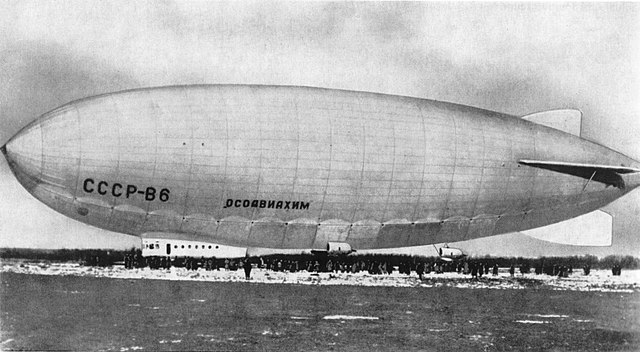
\includegraphics[width=\linewidth]{./chapter/aircraft/airship-SSSR-V6.jpg}}%
}
    \caption{Дирижабль \ruwiki{wKY}{СССР--В6 <<Осоавиахим>>} (1934--1938). 
             Дирижабль В--6 установил мировой рекорд в~1937 году, 
             пролетев 130 с~половиной часов без посадки.
    }%
    \label{fig:airship-stamp}%
\end{marginfigure}
% 
\begin{task}
    \label{answer:aircraft_question_airship_2}
    \newthought{Воздушное судно, изображенное на рис.~\ref{fig:airship-stamp},~--- это дирижабль. Выполнив SPARQL-запрос, представленный на листинге~\ref{lst:aircraft_airship_photo_lst}, можно получить иллюстрации дирижаблей}. 
    
	\begin{lstlisting}[ language=SPARQL, caption={\href{https://w.wiki/t4c}{Изображения дирижаблей}\protect\footnotemark}, label=lst:aircraft_airship_photo_lst, ]
#defaultView:ImageGrid
SELECT ?airship ?airshipLabel ?image
WHERE
{
    ?airship wdt:P31 wd:Q133585. # instance of airship
  	?airship wdt:P18 ?image # image airship
    SERVICE wikibase:label {bd:serviceParam wikibase:language "ru"}
}
\end{lstlisting}
\footnotetext{Получено 18 дирижаблей с иллюстрациями, 2021 год. Ссылка на SPARQL-запрос: \href{https://w.wiki/t4c}{https://w.wiki/t4c} }
    
    \small{Вопрос на с.~\pageref{aircraft_question_5}.}
\end{task}

%%%%%%%%%%%%%%%%%%%%%%%%%%%%%%%%%%%%%%%%%%%%%%%%%%%%

\begin{task}
    \label{answer:prog_lang_1}
    \newthought{Язык программирования \href{https://ru.wikipedia.org/wiki/Ада_(язык_программирования)}{Ада} был разработан Жан Ишбиа, \href{https://ru.wikipedia.org/wiki/Форт_(язык_программирования)}{Форт} разработал Чарльз Мур, а создателем языка \href{https://ru.wikipedia.org/wiki/Erlang}{Erlang} считается Джо Армстронг. Ответ на вопрос также можно получить, выполнив следующий SPARQL-запрос (листинг \ref{lst:prog_lang_answer_1})}. 
	\begin{lstlisting}[language=SPARQL, caption={{\href{https://w.wiki/v4Q}{Создатели языков программирования}}\protect\footnotemark}, label=lst:prog_lang_answer_1]
SELECT ?itemLabel ?developerLabel
WHERE {
 ?item wdt:P31 wd:Q9143
 SERVICE wikibase:label { bd:serviceParam wikibase:language "en,ru" }
 ?item wdt:P178 ?developer.
 SERVICE wikibase:label { bd:serviceParam wikibase:language "en,ru" }
}
ORDER BY DESC (?item_label)
	\end{lstlisting}
\footnotetext{В 2020 году найдено 520 разработчика. Ссылка на SPARQL-запрос: \href{https://w.wiki/v4Q}{https://w.wiki/v4Q}
\newline
\small{Вопрос на с.~\pageref{question:prog_lang_1}.}}
\end{task}

\begin{task}
    \label{answer:prog_lang_2}
    \newthought{Логотипом языка программирования \href{https://ru.wikipedia.org/wiki/LOLCODE}{LOLCODE} является третья картинка. Ответ на вопрос также можно получить, выполнив следующий SPARQL-запрос (листинг \ref{lst:prog_lang_answer_1})}. 
	\begin{lstlisting}[language=SPARQL, caption={{\href{https://w.wiki/v4U}{Логотипы языков программирования}}\protect\footnotemark}, label=lst:prog_lang_answer_1]
#defaultView:ImageGrid
SELECT ?itemLabel ?image
WHERE
{
 SERVICE wikibase:label { bd:serviceParam wikibase:language "en,ru" }
 ?item wdt:P154 ?image. # image
}
	\end{lstlisting}
\footnotetext{В 2020 году получено 87066 логотипов. Ссылка на SPARQL-запрос: \href{https://w.wiki/v4U}{https://w.wiki/v4U}
\newline
\small{Вопрос на с.~\pageref{question:prog_lang_2}.}}

\end{task}

\begin{task}
    \label{answer:prog_langs_4}
    \newthought{Получить список языков программирования со свойством \href{https://www.wikidata.org/wiki/Property:P822}{<<персонаж-талисман>> (P822)} можно выполнив следующий SPARQL-запрос (листинг \ref{lst:prog_lang_answer_4})}. 
	\begin{lstlisting}[language=SPARQL, caption={{\href{https://w.wiki/v4e}{<<Персонажи-талисманы>> языков программирования}}\protect\footnotemark}, label=lst:prog_lang_answer_4]
#List of programming languages with mascot
SELECT ?lang_name ?mascot_name
WHERE {
    ?lang wdt:P31 wd:Q9143 .
    ?lang wdt:P822 ?mascot .
    ?lang rdfs:label ?lang_name filter (lang(?lang_name) = "en").
    ?mascot rdfs:label ?mascot_name filter (lang(?mascot_name) = "en").
}
	\end{lstlisting}
\footnotetext{В 2020 году результат запроса~---~3 языка программирования. Ссылка на SPARQL-запрос: \href{https://w.wiki/v4e}{https://w.wiki/v4e} }
    
    \small{Задание на с.~\pageref{prog_lang_test}.}
\end{task}

\begin{task}
    \label{answer:prog_langs_5}
    \newthought{Получить список языков программирования, основанных ранее 1992 года можно выполнив следующий SPARQL-запрос (листинг \ref{lst:prog_lang_answer_5})}. 
	\begin{lstlisting}[language=SPARQL, caption={{\href{https://w.wiki/v4f}{Языки программирования, старше 1992 года}}\protect\footnotemark}, label=lst:prog_lang_answer_5]
#Select langeages older than 1992
SELECT DISTINCT ?langLabel ?age
WHERE {
  ?lang wdt:P31 wd:Q9143 .
  ?lang wdt:P571 ?age .
  ?lang rdfs:label ?langLabel FILTER (lang(?langLabel) = "ru").
  FILTER(year(?age) < 1992)
}
	\end{lstlisting}
\footnotetext{Результатом запроса в 2020 году были 207 языков. Ссылка на SPARQL-запрос: \href{https://w.wiki/v4f}{https://w.wiki/v4f} }
    
    \small{Задание на с.~\pageref{prog_lang_test}.}
\end{task}

\begin{task}
    \label{answer:prog_langs_6}
    \newthought{Для построения столбчатой диаграммы, отражающуей количество известных хештегов в Твиттере для каждого языка программирования используем свойство (листинг \ref{lst:prog_lang_answer_6})}. 
	\begin{lstlisting}[language=SPARQL, caption={{\href{https://w.wiki/v4h}{Хештеги языков программирования в Твиттере}}\protect\footnotemark}, label=lst:prog_lang_answer_6]
#defaultView:BarChart
#Twitter tags for programming language
SELECT DISTINCT ?langLabel (count(*) as ?count)
WHERE
{
    ?lang wdt:P31 wd:Q9143 .
    ?lang wdt:P2572 ?count .
    ?lang rdfs:label ?langLabel filter (lang(?langLabel) = "ru"). 
} 
GROUP BY ?langLabel
ORDER BY DESC(?count)
	\end{lstlisting}
\footnotetext{Результатом запроса в 2020 году были 3 языка программирования. Ссылка на SPARQL-запрос: \href{https://w.wiki/v4h}{https://w.wiki/v4h} }
    
    \small{Задание на с.~\pageref{prog_lang_test}.}
\end{task}


%%%%%%%%%%%%%%%%%%%  Ship chapter  %%%%%%%%%%%%%%%%%%


\begin{task}
	\label{answer:ship_1}
	Решение:
	\begin{lstlisting}[ language=SPARQL, caption={{\href{https://w.wiki/waV}{Изображения кораблей, снятых в фильмах}}\protect\footnotemark}, label=lst:wide_ship, ]
# Images of ships used in movies
#defaultView:ImageGrid
SELECT DISTINCT ?film ?filmLabel ?ship ?shipLabel ?image
WHERE
{
	?film wdt:P31 wd:Q11424. # is film	
	?film wdt:P921 ?ship . # main subject
	?ship wdt:P31/wdt:P31 wd:Q2235308 . # is ship
	OPTIONAL { ?ship wdt:P18 ?image } # ship's image
								
	SERVICE wikibase:label {bd:serviceParam wikibase:language "ru, en"}
}
	\end{lstlisting}
	\footnotetext{Найдено четыре изображения кораблей, снятых в кинолетнах, 2021 год. Ссылка на SPARQL-запрос: \href{https://w.wiki/waV}{https://w.wiki/waV}}

	\begin{lstlisting}[ language=SPARQL, caption={{\href{https://w.wiki/wXF}{Изображения кораблей, о которых писали в книгах}}\protect\footnotemark}, label=lst:wide_ship, ]
# Images of ships used in movies
#defaultView:ImageGrid
SELECT DISTINCT ?book ?bookLabel ?ship ?shipLabel ?image
WHERE
{
	?film wdt:P31 wd:Q571. # is book	
	?film wdt:P921 ?ship . # main subject
	?ship wdt:P31/wdt:P31 wd:Q2235308 . # is ship
	OPTIONAL { ?ship wdt:P18 ?image } # ship's image
									
	SERVICE wikibase:label {bd:serviceParam wikibase:language "ru, en"}
}
	\end{lstlisting}
	\footnotetext{Найдено пять изображений кораблей, о которых было написано в книгах, 2021 год. Ссылка на SPARQL-запрос: \href{https://w.wiki/wXF}{https://w.wiki/wXF}}
	
\small{Задание на с.~\pageref{question:ship_1}.}
\end{task}


\begin{task}
	На риснуке \ref{fig:grem_answer} изображен советский эсминец~\ruwiki{vgE}{Гремящий}.

	\label{answer:ship_2}
	\begin{marginfigure}[0.0cm]
		{
		  \setlength{\fboxsep}{0pt}%
		  \setlength{\fboxrule}{1pt}%
		  \fcolorbox{gray}{gray}{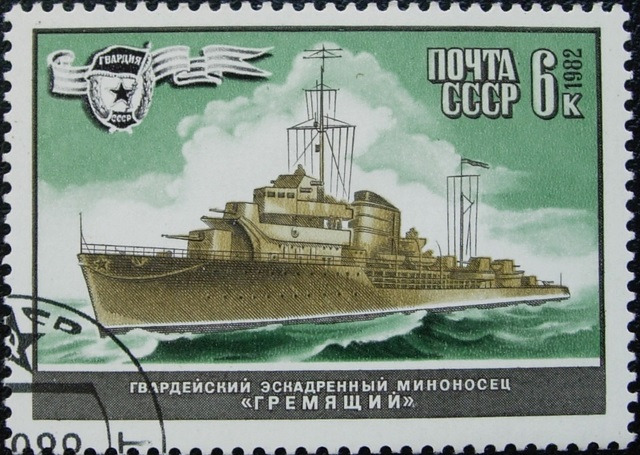
\includegraphics{chapter/ship/Grem_ship_answer.jpg}}
		}
		\caption{Почтовая марка с изображением эсминца~\ruwiki{vgE}{Гремящий}, почта СССР, 1982.}%
		\label{fig:grem_answer}%
	  \end{marginfigure}

    \small{Задание на с.~\pageref{question:ship_2}.}
\end{task}



\begin{task}
	\label{answer:ship_Guinness}
    \newthought{<<Корабли Гиннесса>>}. Поиск самых-самых кораблей по Викиданным.
    \Wikiref{Seawise Giant}~--- это самый длинный нефтяной танкер.

	Примеры возможных решений через Викиданные. Данные могут отличаться от ответа выше из-за неполноты информации об объектах Викиданных, см. листинги~\ref{lst:long_ship} и~\ref{lst:wide_ship}.
\begin{lstlisting}[ language=SPARQL, caption={{\href{https://w.wiki/3L2R}{Самые длинные корабли}}\protect\footnotemark}, label=lst:long_ship,]
# The ship with maximum length
SELECT ?ship ?shipLabel ?max_length WHERE {
	{
		SELECT (MAX(?length) as ?max_length)
		WHERE
		{
			?ship wdt:P31 wd:Q11446; # is ship
				  wdt:P2043 ?length
		}
	}
	{?ship wdt:P31 wd:Q11446; wdt:P2043 ?max_length}
		
	SERVICE wikibase:label { bd:serviceParam wikibase:language "ru, en" }
}  
\end{lstlisting}
\footnotetext{Самым длинным кораблем оказался \Wikiref{NMS Mircea} длиной в \num{3600} метров. Ссылка на SPARQL-запрос: \wwiki{3L2R}}

Внутренний SELECT в скрипте из листинга~\ref{lst:long_ship} находит максимальную длину корабля, а внешний SELECT находит корабль с такой длиной.

\begin{lstlisting}[ language=SPARQL, caption={{\href{https://w.wiki/wKv}{Изображения кораблейm, отсортированные по ширине корабля}}\protect\footnotemark}, label=lst:wide_ship, ]
# List of ships' images sorted by width of ship
#defaultView:ImageGrid
SELECT ?ship ?shipLabel ?image ?beam
WHERE 
{
	?ship wdt:P31 wd:Q11446; # is ship
		  wdt:P2261 ?beam; # width of ship is ?beam
	OPTIONAL { ?ship wdt:P18 ?image }
	SERVICE wikibase:label {bd:serviceParam wikibase:language "ru, en"}
}
ORDER BY DESC(?beam)
\end{lstlisting}
\footnotetext{Самым широким кораблем оказался незавершенный \href{https://www.wikidata.org/wiki/Q1156392}{проект авианосца Хабаккук} из льда и опилок, шириной \num{180} метров, 2021 год. Среди реально существоваших кораблей самым широким оказался норвежский корабль \href{https://www.wikidata.org/wiki/Q11987454}{M/S Isosaari (Q11987454)
}, шириной 99 метров. Ссылка на SPARQL-запрос: \href{https://w.wiki/wKv}{https://w.wiki/wKv}}

\small{Задание на с.~\pageref{question:ship_3}.}
\end{task}

%%%%%%%%%%%%%% spacecraft chapter %%%%%%%%%%%%%%

\begin{task}
    \label{answer:launches_USSR}
    \newthought{Запрос~\ref{lst:launch_USSR} строит график запуска} отечественных космических аппаратов по десятилетиям.
    В 1960-е годы совершено 12 запусков, в 1970-е и 1980-е произведено по 38 запусков.

    \begin{lstlisting}[ 
                language=SPARQL, 
                numbers=none, 
                caption={{\href{https://w.wiki/4QGX}{Диаграмма запусков отечественных космических кораблей по десятилетиям}}\protect\footnotemark}, 
                label=lst:launch_USSR
              ]
# The number of spacecraft launches in Russia every 10 years
#defaultView:BarChart
SELECT (STR(?lapse) AS ?lapse_str) (COUNT(?item) AS ?quantity)
WHERE {                  # spacecraft belongs to
        {?item wdt:P17 wd:Q15180} # Soviet Union
  UNION {?item wdt:P17 wd:Q159}.  # or Russia
  
  ?item wdt:P619 ?launch. # date of spacecraft launch (P619)
  BIND( YEAR(?launch) AS ?year) 
  BIND(FLOOR(?year/10)*10 AS ?lapse) # count for each 10 years
SERVICE wikibase:label {bd:serviceParam wikibase:language "ru,en"}
} 
GROUP BY ?lapse
ORDER BY ?lapse # Order 1960, 1970, 1980, ...    \end{lstlisting}
    \footnotetext{Найдено \num{7} результатов в 2021 г. Ссылка на SPARQL-запрос: \href{https://w.wiki/4dTH}{https://w.wiki/4dTH}}
    \small{Вопрос на с.~\pageref{question:spacecraft_1}.}
\end{task}

\begin{task}
    \label{answer:launches_world}
    \newthought{Наибольшее число запусков за десятилетие в промежуток с 1970 по 2010 год~--- 121, наименьшее~--- 63.} 
    Для подсчёта максимума и минимума запусков за 10 лет в промежуток с 1970 по 2010 год удобно использовать скрипт~\ref{lst:launchesWorld10}.
    \begin{lstlisting}[ language=SPARQL, numbers=none, caption={{\href{https://w.wiki/4dwj}{Максимум и минимум запусков космических кораблей в мире}}\protect\footnotemark}, label=lst:launchesWorld10, ]
# Check MAX and MIN of launches per 10 years from 1970 to 2010
SELECT (MAX (?quantity) as ?max) (MIN (?quantity) as ?min)
WHERE {
  SELECT (STR(?lapse) AS ?lapse_str) (COUNT(?item) AS ?quantity)
  WHERE {                  # spacecraft belongs to
    ?item wdt:P619 ?launch. # date of spacecraft launch (P619)
    BIND( YEAR(?launch) AS ?year) 
    ?item wdt:P17 ?country. # check existing country
    BIND(FLOOR(?year/10)*10 AS ?lapse) # count for each 10 years
    FILTER (?year > 1969 && ?year < 2010) # check date
  } 
  GROUP BY ?lapse
} \end{lstlisting}
    \footnotetext{Запрос выполнялся в 2021 году. Ссылка на SPARQL-запрос: \href{https://w.wiki/4dwH}{https://w.wiki/4dwH}}
    \small{Вопрос на с.~\pageref{question:spacecraft_2}.}
\end{task}

\begin{task}
    \label{answer:spacecraft_USSR}
    \newthought{Космические аппараты}, изображённые на рисунках \ref{question:spacecraft_soyuz19} (Союз--19), \ref{question:spacecraft_soyuzT} (Союз--7К), и \ref{question:spacecraft_lunar} (лунный посадочный модуль <<Космос>>) принадлежат СССР. Убедиться в этом можно выполнив запрос~\ref{lst:imageUSSRsc}:
    \begin{lstlisting}[ language=SPARQL, numbers=none, caption={{\href{https://w.wiki/4eCS}{Набор изображений космических аппаратов СССР}}\protect\footnotemark}, label=lst:imageUSSRsc, ]
# List of images of USSR spacecraft
#defaultView:ImageGrid
SELECT ?obj ?name ?img
WHERE
{
    {?obj wdt:P31 wd:Q40218.}          # spacecraft
    {?obj wdt:P17 wd:Q15180.} UNION       # country
    {?obj wdt:P495 wd:Q15180.}  # country of origin
    ?obj wdt:P18 ?img.                       #image
    OPTIONAL {
		?obj rdfs:label ?name 
		FILTER (lang(?name) = "ru")
	}
}    \end{lstlisting}
    \footnotetext{Найдено девять результатов в 2022 году. Ссылка на SPARQL-запрос: \href{https://w.wiki/4eCS}{https://w.wiki/4eCS}}

    \small{Вопросы на с.~\pageref{question:spacecraft_soyuz19},~\pageref{question:spacecraft_soyuzT},~\pageref{question:spacecraft_lunar}.}
\end{task}

%%%%%%%%%%%%%% Human_settlements charpter %%%%%%%%%%%%%%
\begin{task}
\label{answer:human_settlements_density}
    \newthought{Плотность населения} у Алейска составляет \num{648} чел./км\textsuperscript{2}, 
        у~Барабинска~--- \num{413} чел./км\textsuperscript{2}, 
        то есть у Алейска плотность выше. 

        Плотность населения по населённым пунктам России можно получить 
        с помощью запроса~\ref{lst:human_settlements_density}. 

        Обратите внимание, что площадь может быть задана в разных единицах. 
        Например, у \wdqName{Алейска}{11304591} площадь в Викиданных указана в гектарах, 
        у \wdqName{Барабинска}{104609}~--- в квадратных километрах. 
        Для нормализации данных и перевода площади в метры в 8 строке запроса~\ref{lst:human_settlements_density}
        указан префикс \lstinline|psn:|. 

        Значение переменной \lstinline|?popArea| показывает плотность населения. 
        Во второй строке делим на миллион, чтобы перевести квадратные метры в километры. 

\begin{fullwidth}
\index{SPARQL!psn:!Нормализация площади населённого пункта}
\begin{lstlisting}[ language=SPARQL, 
        caption={\href{https://w.wiki/4duP}{Плотность населения <<населенных пунктов>> России}\protect\footnotemark},
        label=lst:human_settlements_density
                  ]
# population density of human settlements in Russia
SELECT ?hum ?humLabel ?population ?area (?population / (?area / 1000000) as ?popArea) 
WHERE {
  ?hum wdt:P31 wd:Q486972; # instance of human settlement
       wdt:P17 wd:Q159; # in Russia
       
       # Get the area (Use the psn: prefix to normalize the values to a common unit of area)
       p:P2046/psn:P2046/wikibase:quantityAmount ?area;
       
       wdt:P1082 ?population. # has ?population
       FILTER(?population>0 && ?area).
  SERVICE wikibase:label{bd:serviceParam wikibase:language "ru,en"}
}
ORDER BY DESC (?popArea)
\end{lstlisting}
\footnotetext{131 результат на 2021 год. SPARQL-запрос: \href{https://w.wiki/4duP}{https://w.wiki/4duP}}  
\end{fullwidth}

    \small{Вопрос на с.~\pageref{ch:human-settlement}.}
\end{task}

\begin{task}
\label{answer:flag_human_settlements}
\newthought{На рисунках~\ref{fig:flag_question_human_settlements1}, 
    \ref{fig:flag_question_human_settlements2} и 
    \ref{fig:flag_question_human_settlements5}} 
    изображены гербы отечественных населённых пунктов.
    Герб на рис.~\ref{fig:flag_question_human_settlements3} 
    принадлежит населённому пункту \ruwiki{4dUc}{Чехии}, 
    на рис.~\ref{fig:flag_question_human_settlements4}~--- 
    \ruwiki{4dUf}{украинскому} населённому пункту. 

Ответ можно получить с помощью запроса~\ref{lst:flag_question_human_settlements}. 
    Значение свойства  \wdProperty{94}{``coat of arms image''} 
    содержит изображение герба населённого пункта.
   
\index{График!ImageGrid!Гербы населённых пунктов России}
\begin{lstlisting}[ language=SPARQL, 
                    caption={\href{https://w.wiki/4e8A}{Гербы населённых пунктов Российской Федерации}\protect\footnotemark},
                    label=lst:flag_question_human_settlements
                  ]
# Emblems of human settlements in Russia
#defaultView:ImageGrid
SELECT ?hum ?humLabel ?image WHERE {
  ?hum wdt:P31 wd:Q486972; # instance of human settlement
       wdt:P17 wd:Q159;    # in Russia
       wdt:P94 ?image.     # coat of arms
SERVICE wikibase:label{bd:serviceParam wikibase:language "ru, en"}
}
\end{lstlisting}

\footnotetext{148 гербов на 2022 год. SPARQL-запрос: \href{https://w.wiki/4e8A}{https://w.wiki/4e8A}}  
\small{Вопросы на с.~\pageref{fig:flag_question_human_settlements1}, \pageref{fig:flag_question_human_settlements2}, \pageref{fig:flag_question_human_settlements3}, \pageref{fig:flag_question_human_settlements4}, \pageref{fig:flag_question_human_settlements5}.}
\end{task}
